\documentclass[12pt,paper=a4]{article}

\usepackage{graphicx}
\usepackage[margin=3cm]{geometry}
\usepackage{lipsum}
\usepackage[utf8]{inputenc}
\usepackage{amsmath}
\usepackage{indentfirst}
\usepackage{tikz}
\usepackage[bottom]{footmisc}
\usepackage{pgfplots}
\usepackage{array}
\usepackage[hidelinks]{hyperref} 
\usepackage{xcolor}
\usepackage{enumerate}
\hypersetup{
    colorlinks,
    linkcolor={red!50!black},
    citecolor={blue!50!black},
    urlcolor={blue!80!black}
}
\usepackage{pifont}
\usepackage{lastpage}
\usepackage{fancyhdr}
\pagestyle{fancy}
\renewcommand{\headrulewidth}{0pt}
\fancyhead{}
\cfoot{\thepage\ of {\hypersetup{linkcolor=black}\pageref*{LastPage}}}


\begin{document}

\begin{titlepage}
	
	\begin{center}
	
		\noindent\rule{16cm}{0.4pt}\\
		\huge{\bfseries SMART RESTAURANT}\\
		\Large{\bfseries NETWORK AND COMPUTER SECURITY}\\
		\noindent\rule{13cm}{0.4pt}\\
		
		
		\hfill\\
		\textsc{\large Alameda - Group 12}\\
	
		\hfill
	
		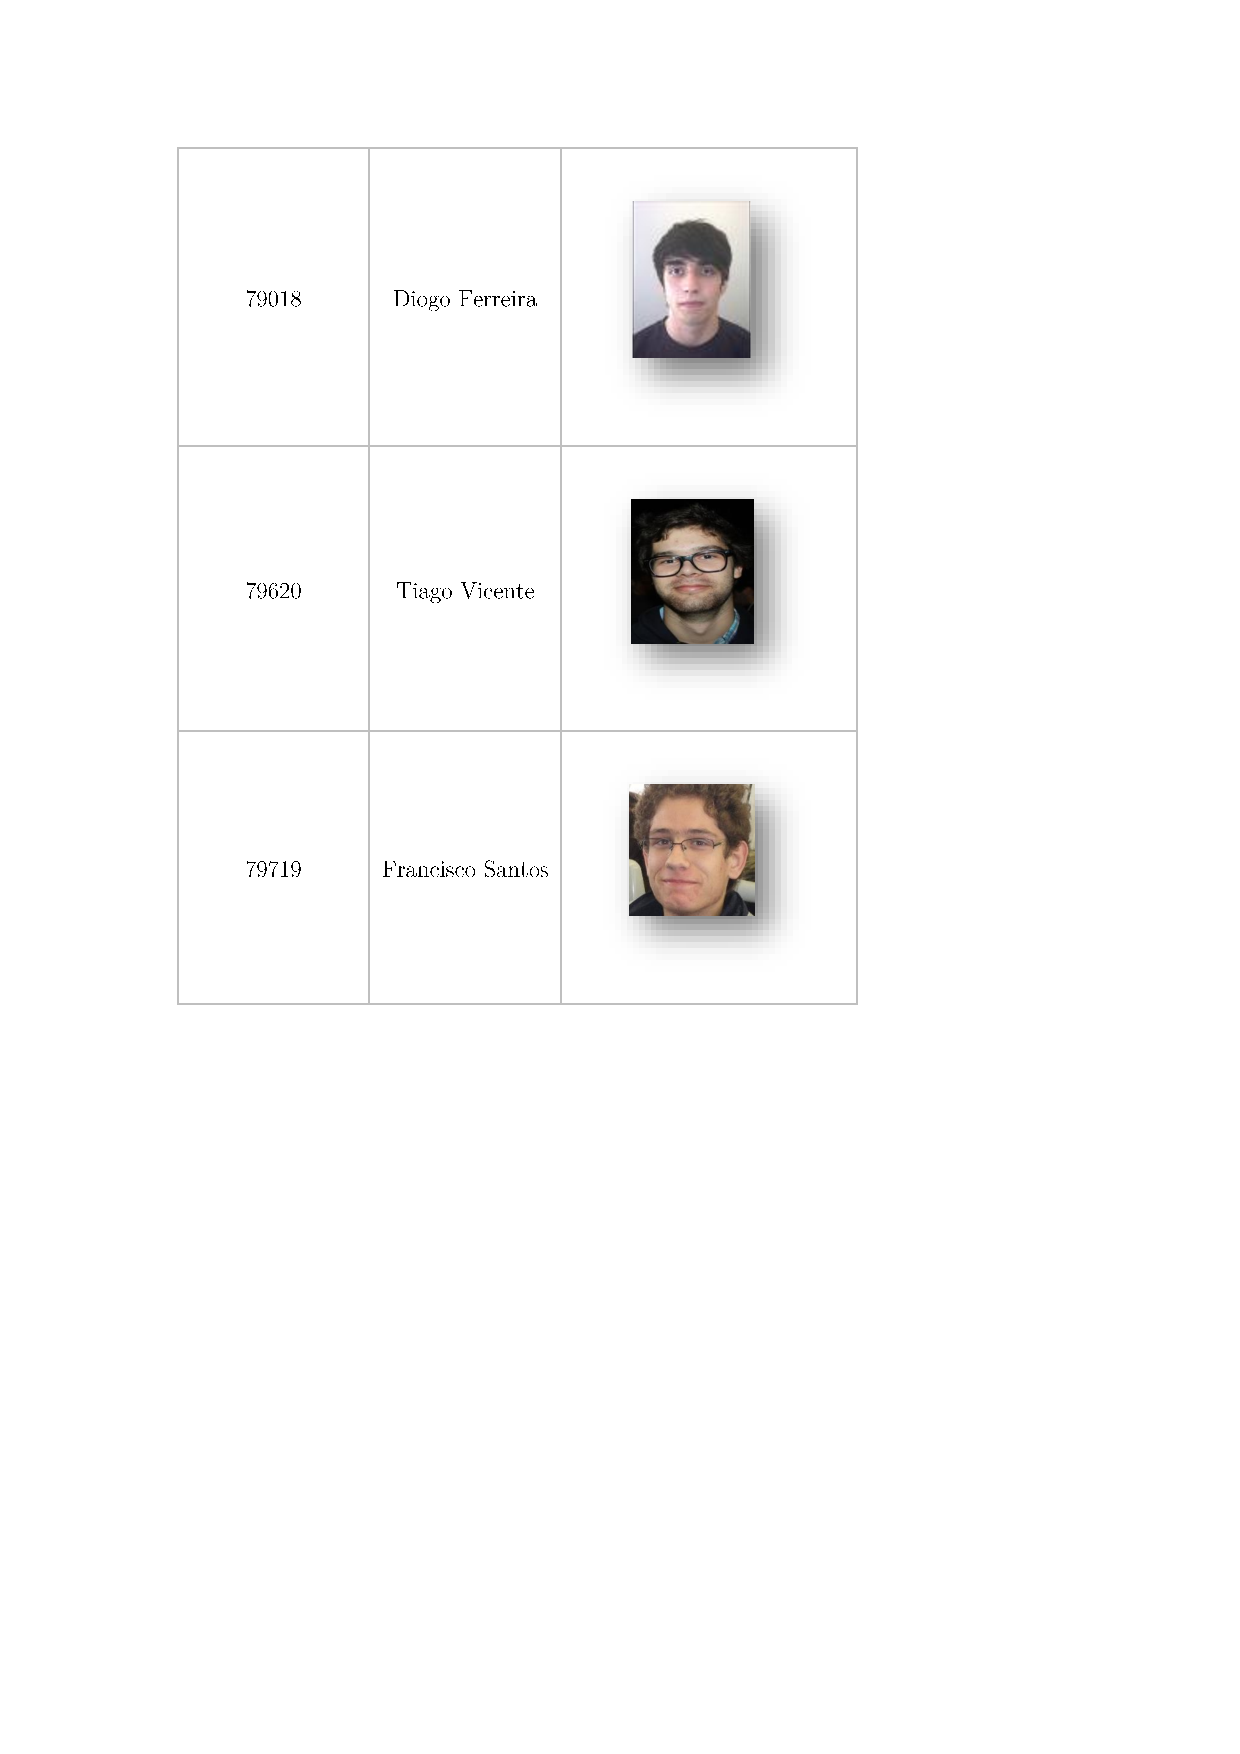
\includegraphics[scale=0.8,trim=-1.1cm 19cm 0 2cm]{Fotos.pdf}
		
		
		\vfill
		\textsc{\small December 09th 2016}\\
		\textsc{\large Instituto Superior Técnico}\\

	\end{center}
	
\end{titlepage}

\section{Problem}
A SmartRestaurant can be everything customers dream for, orders will never be wrong again and they will not be worried about payments again. Although this may seem exciting from the user's point of view, it can be extremely hard to ensure that everything works with high security.

In this case, we will need to make sure that, from the customer side, he cannot be fooled into communicating with a fake restaurant or that someone else is speaking with the server on his behalf, that he can be assured that the order is not tampered with, and that his payment and consumer data is not public. From the restaurant side, it needs to be sure that a client cannot repudiate an order, that their network and infrastructure is not compromised and that there are not clients using their service to attack property of others.

\section{Requirements}
\begin{enumerate}[i]
\item Connection between nodes and server must be secure. Therefore we must assure:
\begin{enumerate}
\item \textbf{Authenticity}: ensure that restaurant’s clients don't make requests on behalf of others;
\item \textbf{Integrity}: avoid tampering with orders made by the clients;
\item \textbf{Freshness}: avoid obsolete orders to be processed;
\item \textbf{Non-repudiation}: guarantee that a client cannot deny making an order;
\item \textbf{Confidentially}: help guarantee integrity and avoid eavesdropping from other clients of: orders or payment data.
\end{enumerate}
\item The service cannot be victim of \textbf{Denial of Service};
\item Protect the network and infrastructures against internal and external attacks due to the mobility of the client's devices;
\item Restaurant clients must have access to the Internet;
\item Outgoing requests must be "\textbf{well behaved}", i.e. don't cause harm to the outside;
\item Clients need to have unique accounts registered in the system;
\item Keep clients records with \textbf{ACID} properties.
\end{enumerate}
\subsection{Assumptions}
The assumptions for the project are: QR Codes cannot be tampered with; smartphones will never be in promiscuous mode; the routing table in the gateway is static; Fénix Framework is safe and for simplicity, a client never cancels an order.
\pagebreak
\section{Proposed solution}

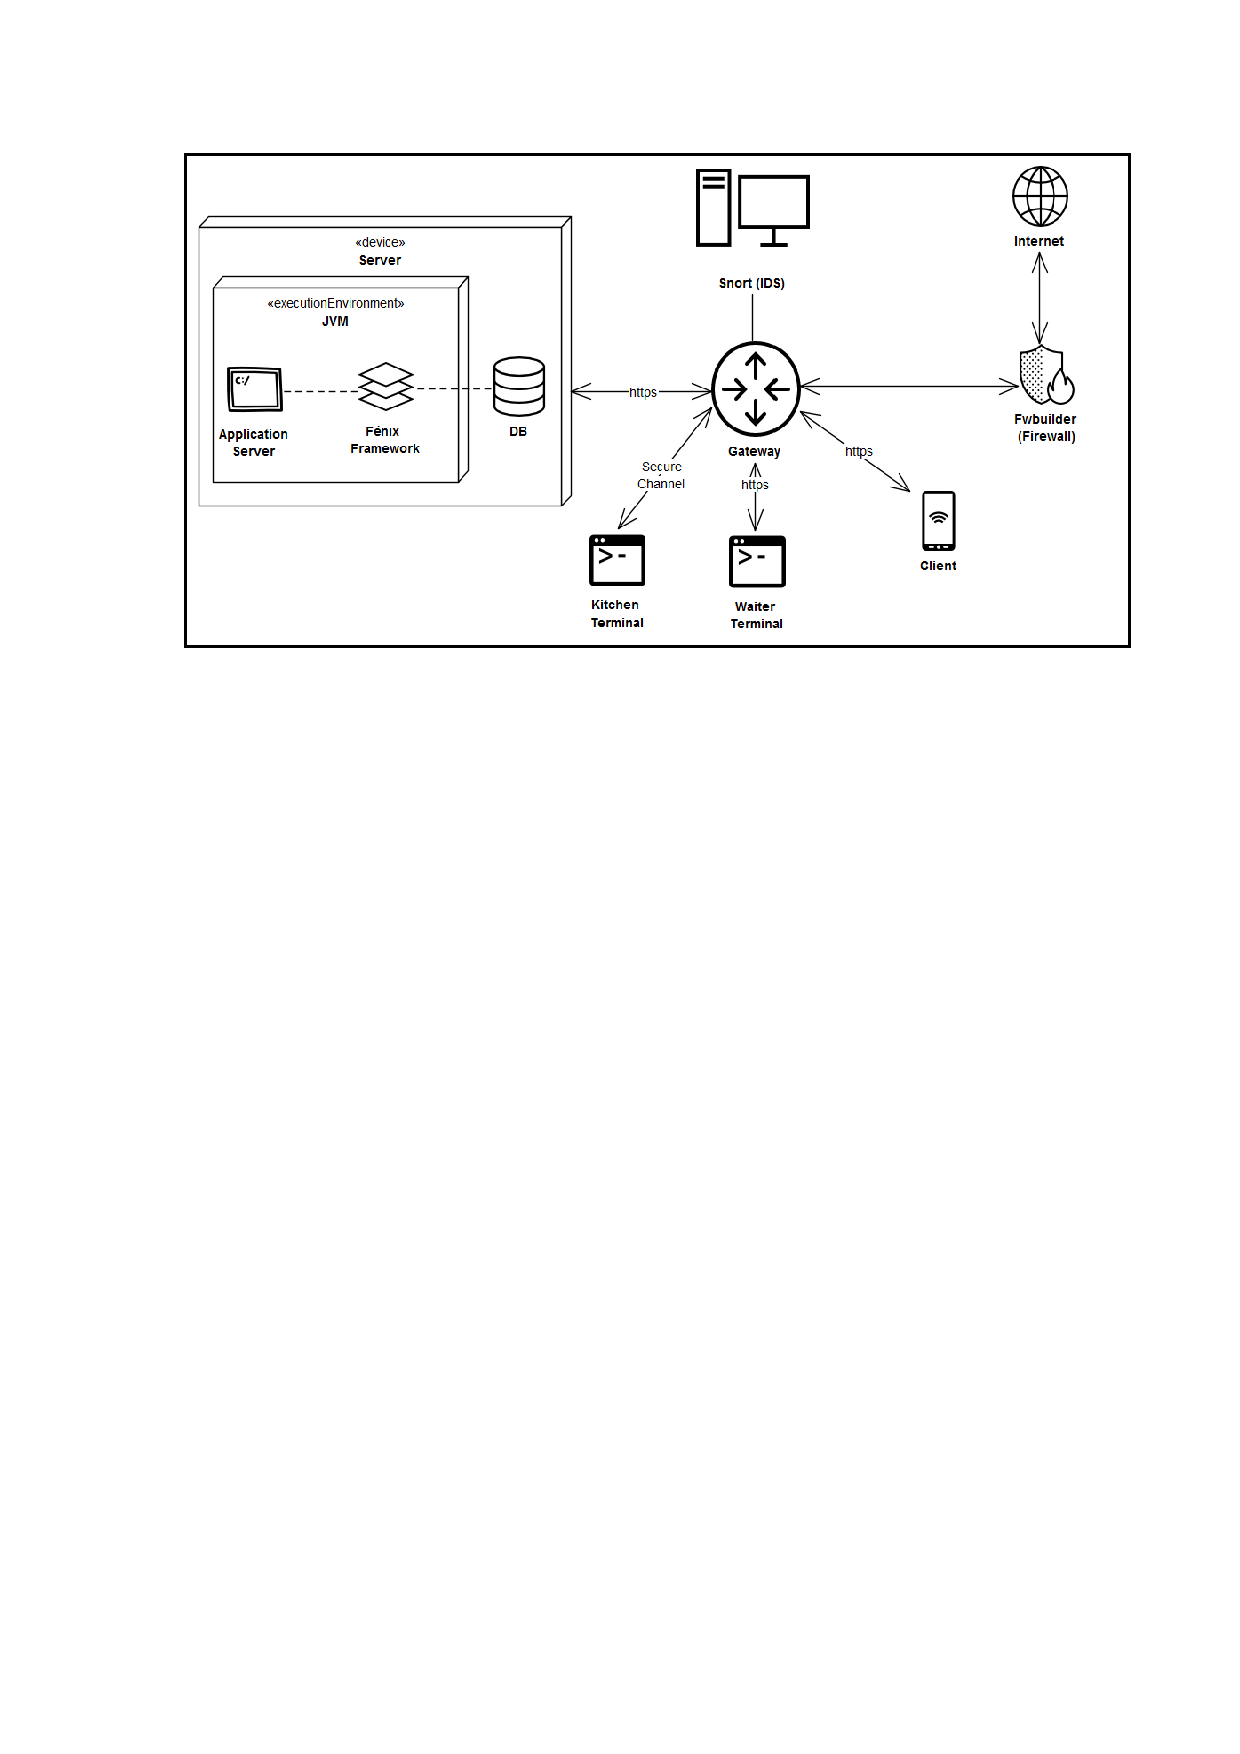
\includegraphics[trim=3.8cm 18cm 0 2cm]{Diagrama.pdf}

The interaction of the system begins with a logged in user reading a QR code, creating a session. The user can make requests using QR codes in the menu. When the user makes a request, it passes through the gateway \textbf{(ii)} where the routing mechanism and IDS come into place. The routing assures that the clients can connect to the server or the outside “world”. \textbf{(iv)} The IDS enforces good internal behavior of the network. \textbf{(iii)}

Once the request from the client reaches the server, it processes the request checking its validity within the business model. The server will use the database to log payments and the amount owed, maintains the state of a request, checks the validity of a user account and on start-up gets the menu QR code translation. \textbf{(vi)} After, the server routes the request to the KitchenTerminal. When ready, it routes back to the server. On the server, it updates the DB setting the request to ready and notifies the WaiterTerminal. The payment is done after the meal is over, recurring to PayPal API.

If the message is directed to the outside the firewall will filter it according to a packet-filter logic \textbf{(v)}. When the response comes, it should behave the same way. \textbf{(iii)}

\subsection{Initial Proposal}
\begin{itemize}
\item[\ding{51}] Application, server and terminals with \textit{Https} connections and sanitization of inputs;
\item[\ding{51}] Notion of user accounts, including creation and payment operations;
\item[\ding{51}] Using QR codes to choose the food and create a session between account-table;
\item[\ding{51}] Database storage for the user accounts, using transactional and persistent domain model;
\item[\ding{51}] Run the system in a local network with no Internet access.
\end{itemize}

\subsection{Intermediate Proposal}
\begin{itemize}
\item[\ding{51}] Implement the connection between the server and the waiters terminal, using the connection requirements \textbf{(i)};
\item[\ding{51}] Configure a Gateway for the internal network in order to intermediate the connection between the clients and the server.
\end{itemize}

\subsection{Final Proposal}
\begin{itemize}
\item[\ding{51}] Configure a Network-based Intrusion Detection System on the gateway;
\item[\ding{51}] Enable Internet access to the client;
\item[\ding{51}] Configure a firewall between the internal network and the external network.
\end{itemize}

\section{Tool references}
The tools that will be used are: \href{https://fenix-framework.github.io/}{Fénix Framework}, \href{https://www.snort.org/}{Snort}, \href{http://www.fwbuilder.org/}{Fwbuilder}, \href{https://jax-ws.java.net/}{JAX-WS}.

\section{Work plan}
\includegraphics[scale=0.85,trim=2.5cm 25cm 0 2cm]{Tabelinha_SIRS.pdf}

\end{document}